%%----------------------------------------------------------------------------
%% Presentatie HoGent Bedrijf en Organisatie
%%----------------------------------------------------------------------------
%% Auteur: Bert Van Vreckem [bert.vanvreckem@hogent.be]

\documentclass{beamer}

%==============================================================================
% Aanloop
%==============================================================================

%---------- Packages ----------------------------------------------------------

\usepackage{graphicx,multicol}
\usepackage{comment,enumerate,hyperref}
\usepackage{amsmath,amsfonts,amssymb}
\usepackage{tikz}
\usepackage[dutch]{babel}
\usepackage[utf8]{inputenc}
\usepackage{multirow}
\usepackage{eurosym}
\usepackage{listings}
\usepackage[T1]{fontenc}
\usepackage{lmodern}
\usepackage{textcomp}
\usepackage{framed}
\usepackage{wrapfig}

%---------- Configuratie ------------------------------------------------------

\usetikzlibrary{arrows,shapes,backgrounds,positioning,shadows}

\usetheme{hogent}

%---------- Commando-definities -----------------------------------------------

\newcommand{\tabitem}{~~\llap{\textbullet}~~}

%---------- Info over de presentatie ------------------------------------------

\title[Intro]{Onderzoekstechnieken\\Les 1. het onderzoeksproces}
\author{Jens Buysse \and Wim {De Bruyn} \and Wim Goedertier \and Bert {Van Vreckem}}
\date{AJ 2017-2018}

%==============================================================================
% Inhoud presentatie
%==============================================================================

\begin{document}

%---------- Front matter ------------------------------------------------------

% Dia met het HoGent logo
\HoGentLogo

% Titeldia met faculteitslogo
\titleframe

%---------- Inhoud ------------------------------------------------------------

\begin{frame}
  \frametitle{Inhoud}

  \tableofcontents
\end{frame}

\section{De wetenschappelijke methode}

\sectionframelogo{\normalsize{\emph{No matter how many instances of white swans we may have observed, this does not justify the conclusion that all swans are white}\\---Karl Popper}}

\begin{frame}
  \scaledimg{img/les1-01}
\end{frame}

\begin{frame}
  \frametitle{Hoe vergaren we kennis?}

  \scaledimg{img/les1-02}
\end{frame}

\begin{frame}[plain,c]
  \begin{columns}
    \column{\dimexpr\paperwidth}
    \includegraphics[width=\paperwidth]{img/les1-03}
  \end{columns}
\end{frame}

\begin{frame}
  \frametitle{Hoe vergaren we kennis?}

  \begin{columns}[c]

  \column{.5\textwidth}
  Niet-wetenschappelijke methode
    \begin{itemize}
    \item ``Mijn buikgevoel zegt van wel''
    \item ``Mijn vader zegt van wel, dus moet het wel''
    \item ``Er zijn verschillende beelden van UFO's en dus kan het niet anders''
    \item ``Ik heb het gelezen op het Internet!''
    \end{itemize}

  \pause

  \column{.5\textwidth}
  Wetenschappelijke methode
    \begin{itemize}
    \item ``Er zijn veel planeten''
    \item ``Moleculen nodig voor leven vind je overal''
    \item $\Rightarrow$ ``Dus ik zou verwonderd zijn indien er geen leven is''
    \item \textbf{Maar er is nog geen bewijs voor}
    \end{itemize}

  \end{columns}
\end{frame}

\begin{frame}
  \frametitle{Kunnen varkens vliegen?}
 % Bedoeling is hier de klas in 3 te delen: ene groep moet aantonen dat varkens kunnen vliegen op autoritaire wijze (bv. Bij boer Mcdonald gaan en navraag), de tweede op deductieve wijze (varkens zijn deel van gewervelden, sommige gewervelden hebben vleugels en dus .. (maar dus met verkeerde conclusie) en de derde tracht dit op wetenschappelijke methode. Hier kan voor deductie ook ik kan in pyama, pyama kan in koffer, dus ik kan in koffer gebruikt worden. 
  \scaledimg{img/les1-04}
\end{frame}

\begin{frame}
  \frametitle{De wetenschappelijke methode}

  Aan de hand van \textbf{empirisch onderzoek} zijn we geïnteresseerd in volgende zaken:

  \begin{enumerate}
    \item Exploratie
    \item Beschrijving
    \item Voorspelling
    \item Controle
  \end{enumerate}
\end{frame}

\begin{frame}
  \frametitle{De wetenschappelijke methode}

  \begin{columns}[c]

    \column{0.8\textwidth}
    \begin{itemize}
      \item Generalisatie
        \begin{itemize}
          \item Bv. ``Agressie komt vaak voor in deze bevolkingsgroep''
        \end{itemize}
      \item Verstaan, begrijpen
        \begin{itemize}
          \item Er is een verband tussen frustratie en agressie
          \item Theorieontwikkeling
        \end{itemize}
    \end{itemize}

    \column{0.2\textwidth}
    \includegraphics[width=\textwidth]{img/les1-05}
    \vspace*{1cm}
    \includegraphics[width=\textwidth]{img/les1-06}

  \end{columns}
\end{frame}

\begin{frame}
  \frametitle{Het onderzoeksproces}

  \begin{columns}
  \column{\dimexpr\paperwidth}
  \begin{center}
    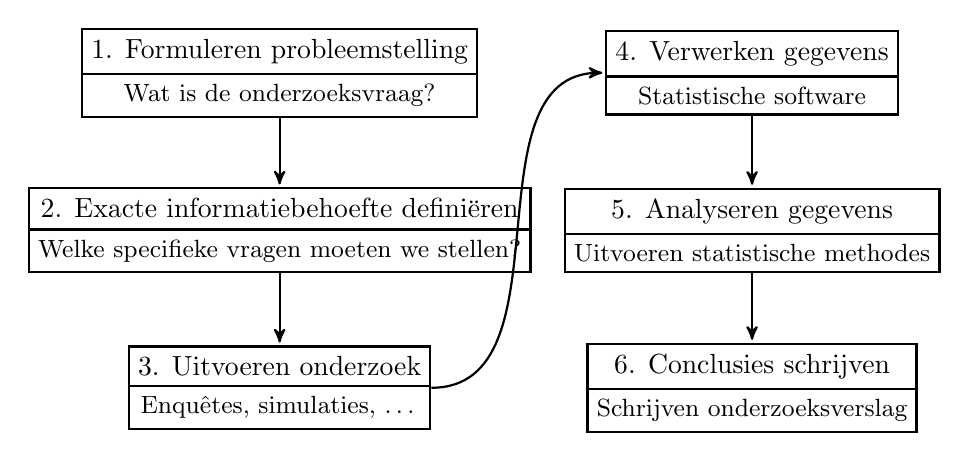
\begin{tikzpicture}[
      auto,
      thick,
      ->,
      >=stealth',
      shorten >=1pt,
      node distance=2cm,
      fase/.style={
        shape=rectangle split,
        rectangle split parts=2,
        ,
        draw}]


      \node[fase] (1) {
        1. Formuleren probleemstelling
        \nodepart{second}
        \small{Wat is de onderzoeksvraag?}
      };
      \uncover<2->{\node[fase] (2) [below of=1] {
        2. Exacte informatiebehoefte definiëren
        \nodepart{second}
        \small{Welke specifieke vragen moeten we stellen?}
      };}
      \uncover<3->{\node[fase] (3) [below of=2] {
        3. Uitvoeren onderzoek
        \nodepart{second}
        \small{Enquêtes, simulaties, \ldots}
      };}
      \uncover<4->{\node[fase] (4) [right of=1, node distance=6cm] {
        4. Verwerken gegevens
        \nodepart{second}
        \small{Statistische software}
      };}
      \uncover<5->{\node[fase] (5) [below of=4] {
        5. Analyseren gegevens
        \nodepart{second}
        \small{Uitvoeren statistische methodes}
      };}
      \uncover<6->{\node[fase] (6) [below of=5] {
        6. Conclusies schrijven
        \nodepart{second}
        \small{Schrijven onderzoeksverslag}
      };}

      \uncover<2->{\draw (1) -- (2);}
      \uncover<3->{\draw (2) -- (3);}
      \uncover<4->{\draw (3.east) to [out=0,in=180] (4.west);}
      \uncover<5->{\draw (4) -- (5);}
      \uncover<6->{\draw (5) -- (6);}
    \end{tikzpicture}
  \end{center}
\end{columns}

\end{frame}

\section{Basisconcepten in onderzoek}

\sectionframelogo{}

\begin{frame}
  \frametitle{Variabelen en waarden}

  \begin{description}
    \item[Variabele] Algemene eigenschap van een object waardoor we objecten van elkaar kunnen onderscheiden
    \item[Waarde] Specifieke eigenschap, invulling voor die variabele
  \end{description}

  \vspace{1cm}

  \begin{columns}[c]
    \column{.6\textwidth}
    \includegraphics[width=\textwidth]{img/les1-07}

    \column{.4\textwidth}
    \fbox{\parbox{3cm}{%
      \scriptsize
      Variabele: geslacht\\
      Waarde: man
    }}\\
    \vspace{.5cm}
    \fbox{\parbox{3cm}{%
      \scriptsize
      Variabele: hoogte\\
      Waarde: 180cm
    }}\\
    \vspace{.5cm}
    \fbox{\parbox{3cm}{%
      \scriptsize
      Variabele: grappig\\
      Waarde: nee
    }}

  \end{columns}
\end{frame}

\begin{frame}
  \frametitle{Meetniveaus}

  Kwalitatieve schalen:

  \begin{description}
    \item[Nominaal] Categorieën. Bv. Geslacht, ras, land, vorm, \ldots
    \item[Ordinaal] Volgorde. Bv. militaire rang, opleidingsniveau, \ldots
  \end{description}

\end{frame}

\begin{frame}
  \frametitle{Meetniveaus}

  Kwantitatieve schalen:

  \begin{description}
    \item[Interval] Meting: getal + meeteenheid, nulpunt niet belangrijk\\
      bv. 20°C - 15°C = 5°C, maar 20°C is \emph{NIET} 1/3 warmer dan 15°C
    \item[Ratio] Meting t.o.v. absoluut nulpunt. bv. Afstand (m), energie (J), massa (kg), \ldots\\
      bv. 20m is \emph{wel} 1/3 langer dan 15m
  \end{description}
\end{frame}

\begin{frame}
  \frametitle{Verbanden tussen variabelen}

  Er is een verband tussen variabelen als hun waarden \textbf{systematisch} veranderen.

  \begin{center}
    \includegraphics[height=4cm]{img/les1-08a}
    \includegraphics[height=4cm]{img/les1-08b}
  \end{center}
\end{frame}

\begin{frame}
  \frametitle{Verbanden tussen variabelen: voorbeeld}

  Is er een verband tussen smaak en cola?

  \begin{columns}
    \column{0.99\textwidth}
    \begin{table}
      \centering
      \begin{tabular}{l||c|c||c}
        & Pepsi & Coca Cola & Totaal \\
        \hline \hline
        Lekker & 56 & 24 & \alert<2>{80} \\
        \hline
        Niet lekker & 14 & 6 & \alert<2>{20} \\
        \hline \hline
        Totaal & \alert<2>{70} & \alert<2>{30} & \alert<2>{100}
      \end{tabular}
    \end{table}

    \only<2>{Marginale totalen}

    \column{.01\textwidth}
    \vspace{4cm}
    \hspace*{-2cm}
%    \begin{wrapfigure}{r}{.3\linewidth}
      \includegraphics[width=2cm]{img/les1-09}
%    \end{wrapfigure}
  \end{columns}
\end{frame}

\begin{frame}
  \frametitle{Oorzakelijke verbanden}

  We zijn vooral op zoek naar \textbf{oorzakelijke verbanden}, bv.

  \begin{itemize}
    \item Frustratie leidt tot agressie
    \item Alcohol leidt tot minder oplettendheid
    \item \ldots
  \end{itemize}

  \begin{description}
    \item[Oorzaak] Onafhankelijke variabele
    \item[Gevolg] Afhankelijke variabele
  \end{description}
\end{frame}

\begin{frame}
  \frametitle{Oorzakelijke verbanden}

  \begin{alertblock}{Let op!}
  Een verband tussen variabelen duidt niet noodzakelijk op een oorzakelijk verband
  \end{alertblock}

  \begin{itemize}
    \item Gaming leidt tot gewelddadig gedrag
    \item Vaccinaties leiden tot autisme
    \item Correlatie tussen drinken van Cola-light en zwaarlijvigheid
    \item \ldots
  \end{itemize}

  \begin{center}
    \includegraphics[height=2.5cm]{img/les1-10}
  \end{center}
\end{frame}

%---------- Back matter -------------------------------------------------------

\end{document}
